% $Id$
%


\section{Arquitectura modelo-vista-controlador}

%%---------------------------------------------------------------

\begin{frame}
\frametitle{�Qu� es la arquitectura MVC?}


\begin{itemize}
\item Patr�n de arquitectura (implementaci�n)
\item Desacopla tres elementos:
  \begin{itemize}
  \item datos (estado de la aplicaci�n)
  \item representaci�n en la interfaz
  \item l�gica de aplicaci�n
  \end{itemize}
\item Modelo: datos (estado) y su gesti�n
\item Vista: Representaci�n en la interfaz (filtrado, actualizaci�n de datos)
\item Controlador: l�gica de la aplicaci�n y flujo de informaci�n
\end{itemize}

\end{frame}

%%---------------------------------------------------------------

\begin{frame}
\frametitle{MVC en aplicaciones web (1)}

\begin{quotation}
The model is any of the logic or the database or any of the data itself. The view is simply how you lay the data out, how it is displayed. [...]

The controller in a web app is a bit more complicated, because it has two parts. The first part is the web server (such as a servlet container) that maps incoming HTTP URL requests to a particular handler for that request. The second part is those handlers themselves, which are in fact often called ``controllers''.[...]
\end{quotation}

\begin{flushright}
``The Importance of Model-View Separation'', Terence Parr \\
\end{flushright}

\end{frame}

%%---------------------------------------------------------------

\begin{frame}
\frametitle{MVC en aplicaciones web}

{\Large
\begin{itemize}
\item Modelo: \\ Descripci�n y gestion de base de datos
\item Vista: \\ Interfaz de usuario (HTML) \\
  que presenta el modelo al usuario
\item Controlador: \\ Recibe indicaciones del usuario, \\
  indica cambios al modelo, \\
  elige vista para mostrar resultados
\end{itemize}
}

\end{frame}

%%---------------------------------------------------------------

\begin{frame}
\frametitle{MVC en applicaciones web}

\begin{center}
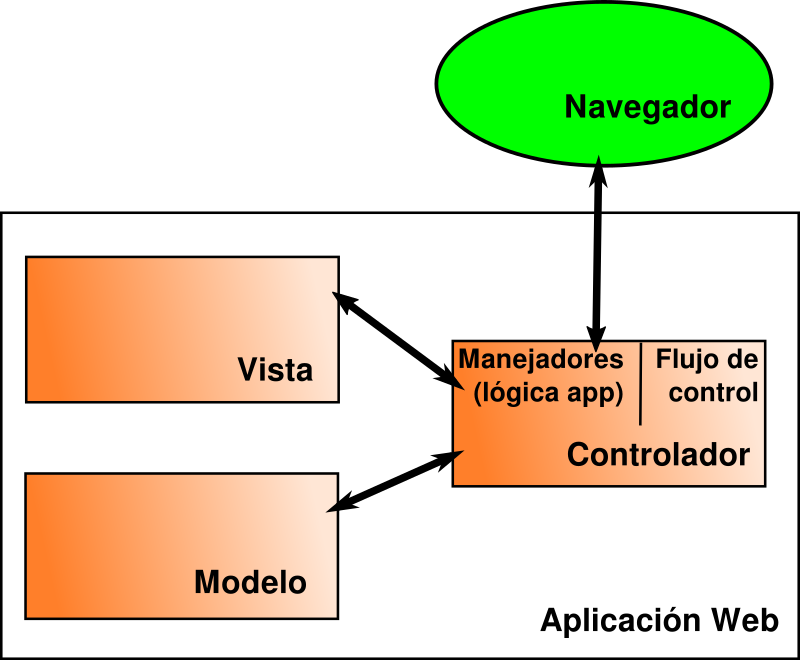
\includegraphics[width=0.8\textwidth]{figs/mvc-basic}
\end{center}
\end{frame}


%%---------------------------------------------------------------

\begin{frame}
\frametitle{MVC en Django}

\begin{itemize}
\item Vista: Manejadores (l�gica de aplicaci�n) \\
  funciones en views.py
\item Vistas delegan la presentaci�n en plantillas (templates)
\item Modelo: Descripci�n de los datos \\
  clases en models.py
\item Controlador: maquinaria de Django \\
  incluyendo urls.py
\item Django como ``plataforma MTV'': \\
  modelo, plantilla (template), vista
\end{itemize}

\end{frame}

%%---------------------------------------------------------------

\begin{frame}
\frametitle{Django: MTV}

\begin{center}
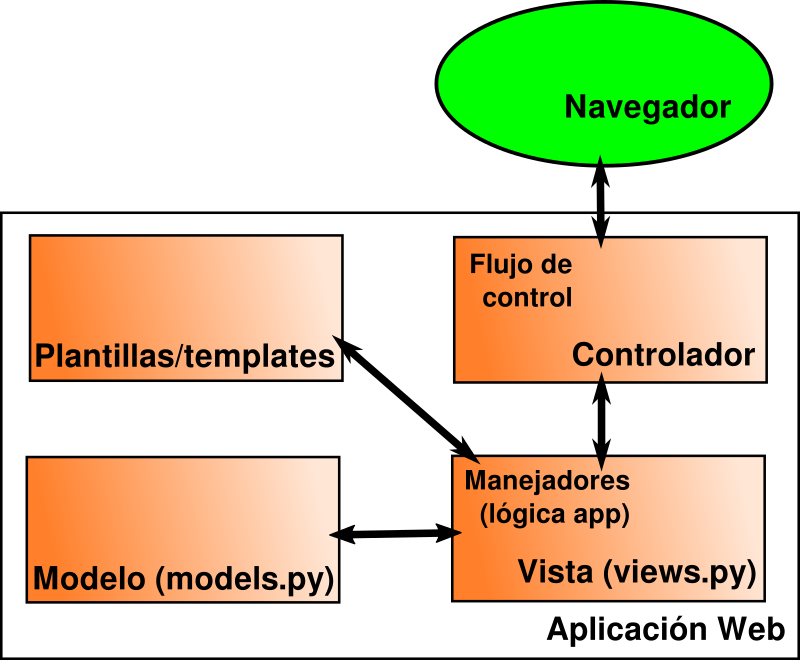
\includegraphics[width=0.8\textwidth]{figs/mvc-mtv}
\end{center}
\end{frame}

%%---------------------------------------------------------------

\begin{frame}
%\frametitle{Django: MTV}

\begin{center}
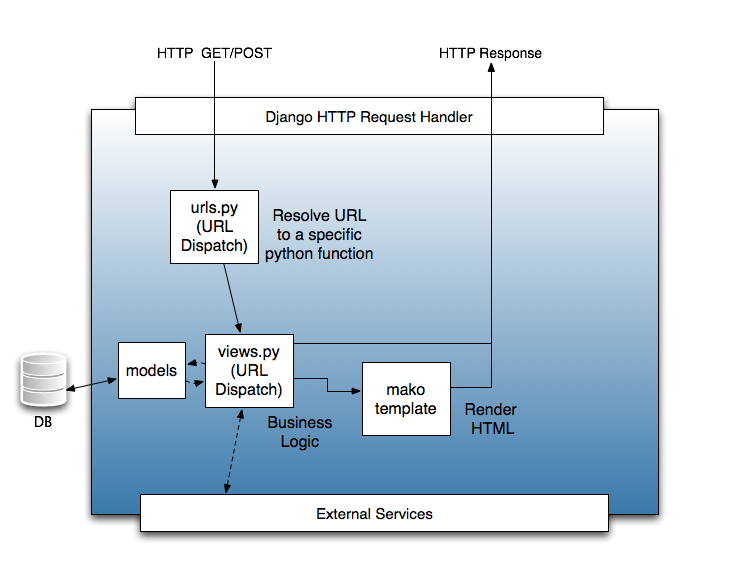
\includegraphics[width=0.85\textwidth]{figs/mvc-mtv-django}
\end{center}

{\footnotesize
Fuente: \url{http://archive.cloudera.com/cdh4/cdh/4/hue/sdk/sdk.html}
}
\end{frame}


%%---------------------------------------------------------------

\begin{frame}
\frametitle{Referencias}

\begin{itemize}
\item MVC, Xerox PARC 1978-79: \\
  \url{http://heim.ifi.uio.no/~trygver/themes/mvc/mvc-index.html}
\item ``The Importance of Model-View Separation. A Conversation with Terence Parr'', by Bill Venners \\
  \url{http://www.artima.com/lejava/articles/stringtemplate.html}
\end{itemize}
\end{frame}
